\section{Karten im Wandel der Zeiten}

\subsection{Babylonische Karte}
\begin{minipage}{8cm}
	\href{http://en.wikipedia.org/wiki/File:Baylonianmaps.JPG}{
	\includegraphics[scale=0.5]{files/images/Baylonianmaps.jpg}}
	\captionof{figure}{Babylonische Karte}
\end{minipage}
\hfill
\begin{minipage}{8cm}
Die älteste bekannte Karte stammt aus Babylonien (6. Jahrhundert v.\,Chr.). Sie befindet sich auf einer Tontafel und wurde
eingeritzt. Die Erde ist eine Scheibe, umgeben von einem Ring -- dem Meer. Im Zentrum befindet sich Babylon umgeben von
anderen Städten. Diese Ritzzeichnung deutet schon die vier Himmelsrichtungen an.\\
\begin{list}{}{}\item[Aufgaben der Karte:]Wiedergabe des Weltbildes\end{list}
\end{minipage}

\subsection{Griechische Karten}
\begin{minipage}{8cm}
	\includegraphics[scale=0.7]{files/images/1-2}
	\captionof{figure}{Griechische Karten}
\end{minipage}
\hfill
\begin{minipage}{8cm}
Bei griechischen Karten befindet sich Griechenland ungefähr im Zentrum.
Die Karten stellen das bekannte bzw. das Erfahrene dar.
Da die Griechen Küstenschiffer waren, sind sie in diesen Bereichen sehr genau.
Man erkennt das Bemühen um Exaktheit (Koordinatensystem).
Es ist eine Erinnerungskarte. Entfernung und folge werden gefühlsmäßig erfasst.
\end{minipage}

\subsection{Römische Karten}
\includegraphics[scale=1]{files/images/1-3}
\captionof{figure}{Römische Karte}
\vspace{0.5cm}

Bei römischen Karten spielt die räumliche Lage eine untergeordnete Rolle.
Interessant war nur die Entfernung zwischen Orten als Maß für die Entfernung wurde ein inneres Maß gewählt.
Die Marschdauer einer Kohorte.

Bei der römischen Karte spielt die Beherrschbarkeit der Entfernung eine Rolle.

\subsection{Die Karten des Mittelalters}
\begin{minipage}{7cm}
Die Karten des Mittelalters enthalten zum einen geografische Details (Kontinente, Flüsse, Städte, Berge, etc.)
und zum anderen spielt die Stellung der Menschen eine bedeutende Rolle.
Dies zeigen Symbole wie \zB Adam und Eva.
Diese Karten spiegeln das religiöse Weltbild.
\end{minipage}
\hfill
\begin{minipage}{8cm}
%\includegraphics[scale=0.7]{files/images/1-4-1}
\href{http://bp1.blogger.com/_gtm0kekxq3U/RhGmLp80wJI/AAAAAAAAADk/cqx1knC8TiY/s320/beatus+wrold+map_spain.JPG}%
{Bild} wegen unklaren Nutzungsrechten aus dem Dokument entfernt.
\captionof{figure}{Karte des Mittelalters}
\end{minipage}

\subsection{Karten der Barockzeit (17./18. Jahrhundert)}
\begin{minipage}{8cm}
	\includegraphics[scale=0.7]{files/images/1-5}
	\captionof{figure}{Karte der Barockzeit}
\end{minipage}
\hfill
\begin{minipage}{8cm}
Die Karte gibt landschaftliche Größenverhältnisse und die relative Lage an.
Objekte, die für den Menschen wichtig sind, werden hervorgehoben.
Sie ist sehr detailliert (Bäume, Städte, Hügel).
Sie ist geeignet zur Orientierung und enthält Informationen, was einen dort erwartet.
\end{minipage}

\subsection{Die Karten der Neuzeit}
\begin{figure}[h!]
	\subfigure{\includegraphics[width=0.49\textwidth]{files/images/1-6-1}}\hfill
	\subfigure{\includegraphics[width=0.49\textwidth]{files/images/1-6-2}}
	\captionof{figure}{Karten der Neuzeit}
\end{figure}
Bei Karten der Neuzeit stehen Lage, Entfernung und Größe der Objekte im Vordergrund.
Häufig werden in einer Karte nur bestimmte Details hervorgehoben.
Es sind also Themenkarten \zB Besitzverhältnisse, Katasterplan, Orientierung --
topografische Karten.

\begin{list}{}{}
	\item[Folgende Entwicklung ist zu beobachten:] Die Empfindung des Menschen zieht sich zunehmend
		zurück und die Abstraktion tritt immer weiter in den Vordergrund.
\end{list}

\section{Die Gedächtniskarte}
\begin{center}
	\includegraphics[scale=0.4]{files/images/Gedaechtniskarte-besser}
	\captionof{figure}{Gedaechtniskarte vom Steinhau Pavilion}
\end{center}

\section{Bezugssysteme}
\begin{list}{}{}
	\item[Unsere Gedächtniskarten gleichen sich in:]~
	\begin{itemize}
		\item Art der Objekte
		\item Lage der Objekte zueinander
		\item Blickrichtung
	\end{itemize}
	\item[Unsere Gedächtniskarten unterscheiden sich in:]~
	\begin{itemize}
	\item Orientierung
	\item Größe
	\end{itemize}
\end{list}

Es ist schwierig, die Lage einzelner Objekte (Häuser, Straßen, etc.) zueinander zu bestimmen.
Deshalb verwendet man in der Landvermessung ein objektunabhängiges Bezugssystem und bestimmt die
Lage zu diesem.

\begin{center}
	\begin{tikzpicture}[color = {black},scale = 1]
		\draw (1,6) -- node [scale=1,sloped,above] {\SI{25}{\metre}} (3.5,3.5)
			-- node [scale=1,sloped,above] {\SI{28}{\metre}} (6.5,0.5);
		\draw (2,2) -- node [scale=1,sloped,above] {\SI{12}{\metre}} (3.5,3.5)
			-- node [scale=1,sloped,above] {\SI{22}{\metre}} (6,6);
	\end{tikzpicture}
	\captionof{figure}{Objektunabhängiges Bezugssystem}
\end{center}

Da die Lage eines Punktes in der Ebene (auch im Raum) nicht definiert werden kann, wird dieses System nie verwendet.

\subsection{Bezugsstrecke}
%%Zeichnung

Zwei festgelegte Punkte ergeben eine Strecke.
Durch zwei Winkel und eine Strecke (WWS, WSW) oder ein Winkel und zwei Strecken (SSW, SWS) oder
kein Winkel und drei Strecken (SSS), kann die Lage jedes beliebigen Punktes zu dieser Strecke
exakt definiert werden.
Diese Strecke nennt man die Bezugsstrecke.
\begin{list}{}{}
	\item[Problem:] Weit entfernte Punkte können nicht erreicht werden.
		$\rightarrow$ Das System muss erweitert werden.
\end{list}

\section{Triangulation}
%%Zeichnung
Sind von einem Dreieck mit drei bekannten Größen (außer WWW), dann ist es exakt definiert.
Alle anderen Größen des Dreiecks (restliche Winkel und/oder Seiten) können berechnet werden (Sinus- und Kosinussatz).
An ein vorhandenes Dreieck werden weitere angegliedert und überziehen die zu vermessende Landschaft.
Es entsteht ein Triangulationsnetz. In dieses Netz können sehr leicht \enquote{Unterdreiecke} eingegliedert werden.

\subsection{Triangulationsnetz}
%%Zeichnung
\begin{list}{}{}
	\item[Problem:] Da sich alle berechneten Werte im Triangulationsnetz auf die Basisstrecke
		beziehen, muss diese extrem genau vermessen werden.
		Denn der Fehler wird in alle folgenden Dreiecke mit hineingerechnet (Multiplikation).
\end{list}

\begin{minipage}{3cm}
	\includegraphics[scale=0.7]{files/images/2-1}
	\captionof{figure}{Triangulationspunkt}
\end{minipage}
\hfill
\begin{minipage}{13.5cm}
Für die Kleinvermessung (Grundstücke, Häuser, etc.) sind die großen Triangulationsnetze in der Regel nicht geeignet, denn
das dazugehörige Großdreieck ist zu weit vom Objekt entfernt. Ein weiteres Problem ist, das manche Objekte nicht in ein
Dreieck gelegt werden können.
\end{minipage}

\section{Polygonzug}
%%Zeichnung
Bei einem geschlossenen Polygonzug legt man kein Netz aus Dreiecken über das Objekt, sondern spannt ein Vieleck auf.
In einem Vieleck können Strecken und Winkel nicht berechnet werden und müssen deshalb alle sehr genau eingemessen werden.
Es gibt auch nur eine direkte Kontrollmöglichkeit, die Winkelsumme.

\vspace{0.5cm}
\begin{tabular}{lll}
\textsc{Fläche} & \textsc{Grad} & \textsc{Gon} \\
\textsc{Dreieck} & \ang{180} & $200^g$ \\
\textsc{Viereck} & \ang{360} & $400^g$ \\
\textsc{Fünfeck} & \ang{540} & $600^g$ \\
\textsc{n-eck} & $(n-2)\cdot \ang{180}$ & $(n-2)\cdot 200^g$ \\
\end{tabular}
\vspace{0.3cm}

In engen Gebirgszügen oder an schwer zugänglichen Orten (\zB Amazonas) kann kein geschlossener Polygonzug gesetzt werden.
Dann muss auf den offenen Polygonzug zurückgegriffen werden.
Bei diesem gibt es keinerlei Kontrollmöglichkeiten, dass heißt die Messungen müssen extrem genau sein.
%%Zeichnung

\subsection{Wie steckt man einen Polygonzug?}
\begin{enumerate}
\item Geländebegehung und Gedächtniskarte zeichnen.
\item Mit Hilfe von Fluchtstäben das Gelände ausstecken (die Fluchtstäbe werden später durch Pflöcke ersetzt.). Die
Fluchtstäbe werden so gesteckt, das man von jedem Punkt den folgenden und den letzten Punkt (Fluchtstabspitze) sieht.
\item Die Strecken sollten nahe an wichtigen zu vermessenden Objekten liegen (nicht parallel), neben Straßen oder quer
darüber.
\item \begin{list}{}{}\item[Es gilt immer:] so viel wie nötig, so wenig wie möglich.\end{list} Lieber drei geschlossene
kleine Polygonzüge als einen großen (Fehlerkontrolle). Bei mehreren Polygonzügen müssen nebeneinanderliegende mindestes
zwei gemeinsame Strecken haben.
\end{enumerate}
%%Zeichnung

\section{Die Längenmessung}
\begin{list}{}{}
	\item[Es gibt folgende Verfahren zur Längenmessung:]~
	\begin{itemize}
		\item Schätzen
		\item Abschreiten
		\item Zeitbedarf
		\item Maßband
		\item Staffelmessung
		\item Laser
		\item GPS
	\end{itemize}
	\item[Ziel:] Die Entfernung zwischen zwei Punkten soll genau bestimmt werden.
		Für die Vogelperspektive braucht man allerdings die projizierte Strecke $e$,
		und nicht die reale $m$.
\end{list}

%%Zeichnung
\begin{list}{}{}
	\item[Problem:] Legt man ein Maßband auf den Boden und P$_1$ und P$_2$ liegen unterschiedlich
		hoch, ist die erfasste Entfernung falsch.
	\item[Weitere Fehler beim Maßband sind:]~
	\begin{itemize}
		\item Dehnungsfehler
		\item Das Durchhängen des Bandes
		\item Kein ebener Untergrund
	\end{itemize}
\end{list}
Ein Maßband ist also zu genauen Messungen ungeeignet.

\vspace{0.5cm}
\ZifferPunktAus
\begin{tabular}{d{0}d{2}d{1}}
	\textsc{Höhe} & \textsc{m} & \textsc{Fehler (\%)} \\
	0 & 10		& 0 \\
	1 & 10,05	& 0,5 \\
	2 & 10,20	& 2 \\
	3 & 10,44	& 4 \\
	5 & 11,18	& 11 \\
\end{tabular}\ZifferPunktAn
$e=\SI{10}{\metre}$
\vspace{0.3cm}

Für eine vernünftige Messung darf der Fehler höchstens 0,02\Prozent{} betragen.

Lösung~\dots
\section{Die Staffelmessung}
\begin{list}{}{}
\item[Bedarfsliste:]~
\begin{itemize}
\item ein Paar 5m Messlatten
\item Meterstab
\item Lattenrichter
\item 2 Lote
\item Fluchtstab
\item 2 (eventuell mehr) Fluchtstabstative
\item Protokollblatt
\item Stift
\item Klemmbrett
\end{itemize}
\item[Durchführung:]
\begin{enumerate}
\item Da die meisten Polygonpunkte zu weit auseinanderliegen,
(mehr als \SIrange{20}{30}{\metre}) müssen zwischen die Polygonpunkte Hilfsstäbe.
\item Auf die beiden Endpunkte der Strecke werden senkrecht zwei Fluchtstäbe gestellt (oder direkt in die Flucht dahinter)
und mithilfe der Fluchtstabstative fixiert.
\item Zwischen die beiden Polygonpunkte werden nun im Abstand von \SIrange{20}{30}{\metre} Hilfsstäbe eingefluchtet.
Eine Person steht \SIrange{1}{2}{\metre} hinter dem Polygonpunktfluchtstab und peilt an der rechten Seite vorbei.
Eine zweite Person hält einen Fluchtstab \enquote{frei schwebend} (er hält ihn am oberen Ende) ist er in der Flucht, wird
er gesteckt.
\begin{list}{}{}\item[Achtung:] Die Entfernung zu diesen Hilfsstäbem wird nicht erfasst.\end{list}
\begin{picture}(30,38)
%\linethickness{1mm}
\put(20,20){\line(1,0){120}}%Senkrecht
\put(35,17){\makebox(1,0){P$_1$}}
\put(125,17){\makebox(1,0){P$_2$}}
\put(60,26){\makebox(1,0){H$_1$}}
\put(95,26){\makebox(1,0){H$_2$}}
\put(77,30){\makebox(1,0){Fluchtstäbe}}
\put(77,17){\makebox(1,0){Sehstrahl}}
\put(15,16){\makebox(1,0){Auge}}
%\put(11,15.5){\circle*{0.8}}
\put(18,20){\circle*{3}}
\put(30,21.5){\circle{3}}
\put(35,21.5){\circle{3}}
\put(94.5,21.5){\makebox(1,0){x}}
\put(59.5,21.5){\makebox(1,0){x}}
\put(60,21.5){\circle{3}}
\put(95,21.5){\circle{3}}
\put(125,21.5){\circle{3}}
\end{picture}

\begin{center}
%\captionof{figure}{Eingefluchten von Fluchtstäben}\vspace{0.5cm}

	\includegraphics[scale=0.8]{files/images/2-2}

	\includegraphics[scale=0.8]{files/images/2-3}
	\captionof{figure}{Veranschaulichungen der Längenmessung}
\end{center}
\vspace{0.5cm}
Mit der Messung beginnt man am besten am oberen Punkt. (Entspricht Hinmessung). Die Rückmessung macht man dann bergauf.
\item Messlatte hochkant genau auf den Polygonpunkt setzen und fixieren (Person 1) -- Person 2 hält das andere Lattenende
(ungefähr waagrecht).
\item Messlatte in die Waagrechte bringen und grob in die Flucht legen.
\item Messlatte genau einfluchten.
\item Messlatte perfekt in die Waagerechte bringen (man kann einen Fluchtstab zum Fixieren nehmen)
\item Am \enquote{frei schwebenden} Ende wird jetzt das Lot über die Metallklappe gefällt (Person 4)
\item Die zweite Messlatte genau an der Lot spitze fixieren (liegt auf dem Boden), grob in die Waagerechte bringen und in
die Flucht legen (Person 5 und 6) jetzt die zweite Latte genau einfluchten und in die Waagerechte bringen.
\item Das Lot am Ende der zweiten Latte fällen.
\item Die erste Latte kann jetzt entfernt werden und wird vom Protokollanten notiert. Notiert wird w (weiß) bzw. r (rot).
Jetzt wird diese Latte an die Lotspitze von Latte zwei gelegt.
\item Diesen Vorgang wiederhold man so oft, bis man mit der letzten Latte über dem zweiten Polygonpunkt ist. Das letzte
Stück wird jetzt mit dem Meterstab auf der letzten Latte gemessen (mm genau).
\item Jetzt folgt die Rückmessung. Das Messprinzip ist das Gleiche, nur muss das Lot von der nächsten Latte zurück gefällt
werden.\begin{list}{}{}\item[Achtung:] Immer auf die Waagrechte und die Flucht achten!\end{list}
Die Differenz sollte nicht größer als \SI{2}{\centi\metre} auf \SI{100}{\metre} sein.
\begin{list}{}{}\item[Ist sie größer, dann:]~
\begin{itemize}
\item auf keinen Fall die Zahlen zurecht mogeln. Denn man weiß nicht, welche Messung falsch war.
\item Hinmessung oder Rückmessung Wiederholung, bei der man ein schlechtes Gefühl hat.
\item Keine Messergebnisse wegstreichen!
\end{itemize}
\end{list}
\end{enumerate}
\end{list}

\section{Die Höhenmessung}
\begin{list}{}{}
%\item[1. Problem:]
%Zeichnung
\item[1. Problem:] %2
%Zeichnung
Diese gelbe Strecke ist eigentlich eine Ebene.
Es ist die Tangentialebene parallel zur Erdoberfläche.
Es ist eine optische Ebene.
\end{list}

\subsection{Fehler Erdkrümmung}
\vspace{0.5cm}
\begin{center}
\begin{tikzpicture}[color = {black},scale = 1]
	\draw (5,5) circle (3);
	\draw (1,8) -- (9,8);
	\draw (5,5) -- (5,8);
	\node[scale = 1] at (5.15,6.5) {$r$};
	\node[scale = 1.4] at (5,3) {Erdkörper};
\end{tikzpicture}
\captionof{figure}{Der Effekt der Erdkrümmung}
\end{center}
\vspace{0.5cm}

\begin{tabular}{ll}
\textsc{Entfernung} & \textsc{Fehler} \\
\SI{100}{\metre} & \SI{0,8}{\milli\metre} \\
\SI{500}{\metre} & \SI{2}{\centi\metre} \\
\SI{1}{\kilo\metre} & \SI{7,9}{\centi\metre} \\
\SI{5}{\kilo\metre} & \SI{1,96}{\metre} \\
\SI{200}{\kilo\metre} & \SI{4807}{\metre} \\
\end{tabular}

%\vspace{0.3cm}\begin{list}{}{}\item[Bedarfsliste:]
%\begin{itemize}
%\item Ein
%\end{itemize}
%\end{list}


\section*{Hier fehlt etwas Text~\dots}

\begin{center}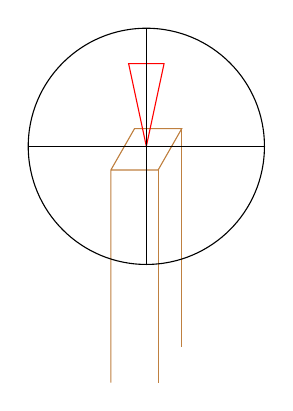
\begin{tikzpicture}[color = {black},scale = 1.5]
\draw[color = brown] (-0.3,-2) -- (-0.3,-0.2) -- (-0.1,0.15) -- (0.3,0.15) -- (0.1,-0.2) -- (-0.3,-0.2);
\draw[color = brown] (0.1,-0.2) -- (0.1,-2);
\draw[color = brown] (0.3,0.15) -- (0.3,-1.7);
\draw[color = red] (0,0) -- (-0.15,0.7) -- (0.15,0.7) -- (0,0);
\draw (-1,0) -- (1,0);
\draw (0,-1) -- (0,1);
\draw (0,0) circle (1);
\end{tikzpicture}\end{center}
\captionof{figure}{Anpeilen einer Fluchtstab Spitze}

\begin{center}\begin{tikzpicture}[color = {black},scale = 1.4]
%%Rechtes Dreieck
\draw[green] (2,3) -- (2,6) -- (0,6);
\draw (1,5) -- (1,7) -- (3,5) -- (1,5);
%%Linkes Dreieck
\draw[green] (4.4,3) -- (4.4,6) -- (6.4,6);
\draw (3.4,5) -- (5.4,5) -- (5.4,7) -- (3.4,5);
%%
%\draw (1.5,3) -- (2.5,3) -- (2.5,2.4) -- (1.5,2.4) -- (1.5,3);
%%
\draw[green] (3.2,3) -- (3.2,7);
\end{tikzpicture}\end{center}\captionof{figure}{Funktionsweise eines Winkelprismas}\vspace{0.5cm}

\begin{center}\begin{tikzpicture}[color = {black},scale = 1.4]
\draw[red] (0.3,7) -- (0.3,7.33);\draw[red] (0.5,7.33) -- (0.5,7.66);\draw[red] (0.7,7.66) -- (0.7,8);
\draw[blue] (0,8) -- (1,8) -- (1,7) -- (0,7) -- (0,8) -- (0,7.66) -- (1,7.66) -- (1,7.33) -- (0,7.33);
\draw[red] (2,7.2) -- (4,7.2);\node[scale = 0.7,red] (X) at (2,7.2) {X};\node[scale = 0.7,red] (X) at (4,7.2)
{X};\node[scale = 0.7,red] (X) at (3,7.9) {X};
%
\draw[red] (0.5,5) -- (0.5,5.33);\draw[red] (0.3,5.33) -- (0.3,5.66);\draw[red] (0.5,5.66) -- (0.5,6);
\draw[blue] (0,6) -- (1,6) -- (1,5) -- (0,5) -- (0,6) -- (0,5.66) -- (1,5.66) -- (1,5.33) -- (0,5.33);
\draw[red] (2,5.2) -- (4,5.2);\node[scale = 0.7,red] (X) at (2,5.2) {X};\node[scale = 0.7,red] (X) at (4,5.2)
{X};\node[scale = 0.7,red] (X) at (3,5.9) {X};\node[scale = 0.9,green] (X) at (3.3,5.2) {X};\node[scale = 0.9,green] (X)
at (3,7.6) {X};
%
\draw[red] (0.5,3) -- (0.5,4);
\draw[blue] (0,4) -- (1,4) -- (1,3) -- (0,3) -- (0,4) -- (0,3.66) -- (1,3.66) -- (1,3.33) -- (0,3.33);
\draw[red] (2,3.2) -- (4,3.2);\node[scale = 0.7,red] (X) at (2,3.2) {X};\node[scale = 0.7,red] (X) at (4,3.2)
{X};\node[scale = 0.7,red] (X) at (3,3.9) {X};\node[scale = 0.9,green] (X) at (3,3.2) {X};
\end{tikzpicture}\end{center}\captionof{figure}{Zurechtfinden mit einem Winkelprismas}

\section{Höhenlinien}
Durch die Höhenmesstrupps wird zuerst die Höhe jedes Polygonpunktes erfasst.
Man misst immer auf den Pflöcken, der Fehler (Pflockhöhe) wird später korrigiert.
Die Qualität der Messung, also die Kontrolle, erfolgt durch das Aufsummieren der Einzelhöhen.
Die Summe innerhalb eines Polygonzuges ist immer 0.
\enquote{Einmal} wird die offizielle Höhe von der Höhenmarke zu einem Pflock bestimmt.
So kann die absolute Höhe jedes Polygonpunktes exakt angegeben werden.

\begin{center}
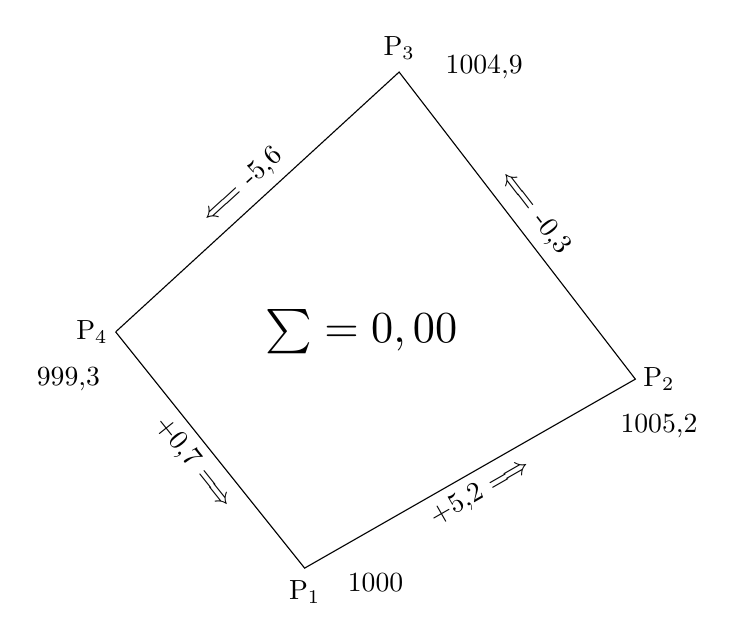
\begin{tikzpicture}[color = {black},scale = 0.6]
	\node[scale = 1.6] (P4) at (5.2,5) {$\sum = 0,00$};
	\node[scale = 1] (P4) at (-0.5,5) {P$_4$};
	\node[scale = 1] (P3) at (6,11) {P$_3$};
	\node[scale = 1] (P2) at (11.5,4) {P$_2$};
	\node[scale = 1] (P1) at (4,-0.5) {P$_1$};
	\node[scale = 1] (P4h) at (-1,4) {\SI{999,3}{\metre}};
	\node[scale = 1] (P3h) at (7.8,10.6) {\SI{1004,9}{\metre}};
	\node[scale = 1] (P2h) at (11.5,3) {\SI{1005,2}{\metre}};
	\node[scale = 1] (P1h) at (5.5,-0.3) {\SI{1000}{\metre}};
	\draw (0,5) -- node [scale=1,sloped,above] {$\Longleftarrow$ \SI{-5,6}{\metre}}  (6,10.5) --
		node [scale=1,sloped,above] {$\Longleftarrow$ \SI{-0,3}{\metre}} (11,4) --
		node [scale=1,sloped,below] {$+$\SI{5,2}{\metre} $\Longrightarrow$} (4,0) --
		node [scale=1,sloped,below] {$+$\SI{0,7}{\metre} $\Longrightarrow$} (0,5);
\end{tikzpicture}
\captionof{figure}{Höhenlinien durch einen Polygonzug}
\end{center}

Die \SI{1000}{\metre} Höhenlinie läuft durch P$_1$.
Die \SI{1002,5}{\metre} Höhenlinie verläuft zwischen P$_1$ \& P$_2$ und P$_3$ \& P$_4$.
%% Ich weiß, dass "&" Typographisch unpassend ist ...
Die \SI{1005}{\metre} Höhenlinie verläuft zwischen P$_2$ \& P$_3$ und P$_1$ \& P$_2$.

\newpage
\section{Tachymetrie}
tachys \entspricht schnell

Mit Hilfe der Tachymetrie, kann mit einem Theodoliten der Winkel, die Höhe und die Entfernung mit einem einzigen
Messvorgang bestimmt werden.

\subsection{Messung der Entfernung}
\begin{center}
\begin{tikzpicture}[color = {black},scale = 1.6]
\draw (0,2) -- (8,2) -- (8,5);
\node[scale = 1] (Hml) at (8,5.3) {Höhenmesslatte};
\draw (1,0.75) -- (1,1.45) -- (1,1.1) -- node [scale=1,sloped,above] {$e$} (8,1.1) -- (8,0.75) -- (8,1.45);
\draw (1,2) -- (1,2.7) -- (0.7,2);\draw (1,2.7) -- (1.3,2);
\node[scale = 1] (P1) at (1,1.7) {P$_1$};
\node[scale = 1] (P2) at (8,1.7) {P$_2$};
\draw (0.65,2.7) -- (0.65,3) -- node [scale=1,sloped,above,green] {$e'$} (1.35,3) -- (1.35,2.7) -- (0.65,2.7);
\node[scale = 1,red] (t') at (1.5,3.1) {$t'$};
\draw (0.3,2) -- node [scale=1,sloped,above] {\SI{1,5}{\metre}} (0.3,2.85) -- (0.2,2.85) -- (0.4,2.85);
\draw[yellow] (0.65,2.85) -- (8,3.5);
\node[scale = 1] (3.5) at (8.35,3.5) {\SI{2,5}{\metre}};
\draw[yellow] (0.65,2.85) -- (8,2.85);
\node[scale = 1] (e) at (6,2.98) {$e$};
\node[scale = 1] (2.85) at (8.35,2.85) {\SI{1,5}{\metre}};
\draw (7.93,3.12) arc (90:180:0.2);\draw[fill=black] (7.88,2.97) circle (0.02);
\draw[yellow] (0.65,2.85) -- (8,2.2);
\draw[green] (0.65,2.85) -- (1.35,2.85);\draw[red] (1.35,2.923) -- (1.35,2.777);
\node[scale = 1] (2.2) at (8.35,2.2) {\SI{1,5}{\metre}};
\node[scale = 5.6] (2.2) at (8.95,2.85) {\}};
\node[scale = 1] (2.2) at (9.8,2.85) {\SI{2}{\metre} = $t$};
\end{tikzpicture}
\captionof{figure}{Messung der Entfernung mithilfe eines Theodoliten}
\end{center}

\begin{align}
\frac{e}{t} &= \frac{e'}{t'}\quad\vert \cdot t \\
e &= \frac{e'}{t'}\cdot t \\
\frac{e'}{t'} &= 100\;\text{(Werkseitig eingestellt)} \\
e &= 100\cdot t \\
e &= 2\cdot 100 \\
e &= \uuline{\SI{2}{\metre}}
\end{align}\setcounter{equation}{0}

\subsection{Messung der Höhe}
\begin{center}
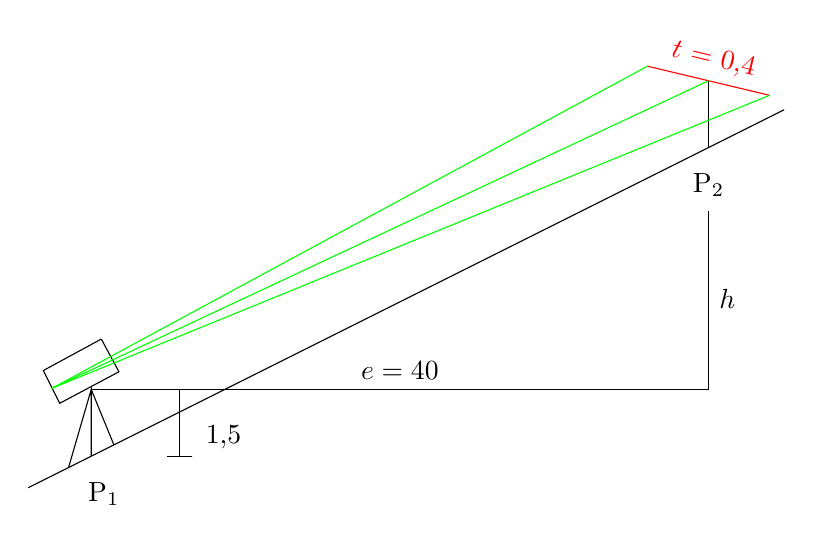
\begin{tikzpicture}[color = {black},scale = 1.6]
\draw (0,2) -- (6,5); %0,0 6,3
\draw (0.32,2.16) -- (0.5,2.78) -- (0.5,2.25);
\draw (0.5,2.78) -- (0.68,2.34);
\draw (0.58,3.18) -- (0.12,2.93) -- (0.25,2.67) -- (0.72,2.92) -- (0.58,3.18);
\node[scale = 1] (P1) at (0.6,1.95) {P$_1$};
\node[scale = 1] (P2) at (5.4,4.4) {P$_2$};
\draw[red] (4.8,5.23,-0.3) -- node [scale=1,sloped,above] {$t$ = \SI{0,4}{\metre}} (6,5.23,0.3);
%\node[scale = 1,red] (P2) at (5.5,5.5) {$t$ = 0,40m};
\draw (0.5,2.78) -- node [scale=1,sloped,above] {$e = \SI{40}{\metre}$} (5.4,2.78) -- (5.4,4.2);
\node[scale = 1] (h) at (5.55,3.5) {$h$};
\draw (5.4,5.23) -- (5.4,4.7);
\draw[green] (0.19,2.79) -- (5.4,5.23);
\draw[green] (0.19,2.79) -- (6,5.23,0.3);
\draw[green] (0.19,2.79) -- (4.8,5.23,-0.3);
\draw (1.2,2.78) -- (1.2,2.25) -- (1.3,2.25) -- (1.1,2.25);
\node[scale = 1] (t') at (1.55,2.4) {\SI{1,5}{\metre}};
\end{tikzpicture}
\captionof{figure}{Messung der relativen Höhe mithilfe eines Theodoliten}
\end{center}

\begin{align}
\tan \alpha &= \frac{h}{e} \\
\tan \alpha &= \frac{h}{40}\quad\vert \cdot 40 \\
h &= \tan \alpha \cdot 40 %\\
%e &= \uuline{200cm}
\end{align}
